\chapter{Domain Driven Design}

Domain-Driven design (DDD) is the concept that the structure and language of your code (class names, class methods, class variables) should match the business domain. DDD objective is to ease the creation of complex applications by connecting the related pieces of the software into an evolving model. Generally DDD is the architectural approach that is used to design large system. The guidelines used by DDD are highly compatible with those reactive architecture so as a result you'll often see them used together.

\section{Domain}

A domain is a sphere of knowledge. In the context of software, it refers to the business idea that we are modeling. A domain is defined by the Domain-Experts that understand the business idea, but not necessarily the software. The key goal of DDD is to build a model that the domain experts can understand. So we can conclude:
\begin{itemize}
    \item The model represents our understanding of the domain;
    \item The software is an implementation of the model.
\end{itemize}

\section{Ubiquitous Language}

Ubiquitous Language is the term by Eric Evans in order to build a language shared by the team, developers, domain experts, and other participants.
Regardless of how software is designed, it will need to reflect a clear and modeled Ubiquitous Language within a Delimited Context. Ubiquitous Language (UL) has the following characteristics:
\begin{itemize}
    \item Must be expressed in the Domain Model:
    \begin{itemize}
        \item Terminology in the UL comes from the domain experts;
        \item Words originate in the domain and are used in the software;
        \item Avoid taking software terms and introducing them into the domain;
        \item Domain Experts and Developers should be able to have a conversation without resorting to software terms. 
    \end{itemize}
    \item Unites the people of the project team;
    \item Eliminates inaccuracies and contradictions from domain experts;
    \item Not a business language imposed by domain experts or a language used in industries;
    \item Evolves over time, it is not define entirely in a single meeting;
    \item Concepts that are not part of the Ubiquitous Language should be rejected.
\end{itemize}

\section{Subdomains}

We can say that Domain is a scope where one works and how one works, in the other words, it refers to the space of the problem for which we are acting, its entities, behaviors and rules. It is from the Domain that we design our Domain Models, which solutions that seek to meet the needs of the domain. It is a mistake that we can create a single Domain Model. If you try to do that it will surely fail. 
We can see a restaurant domain in the Figure~\ref{fig:domain} as example.

\begin{itemize}
    \item Business Domains are often large and complicated;
    \item They contain many ideas, actions and rules that interact in complex ways;
    \item Trying to model a large domain can become problematic;
    \item Therefore, we separate our large domains into subdomains.
\end{itemize}

\begin{figure}[ht]
\caption{Example of a Restaurant Domain}
\centering
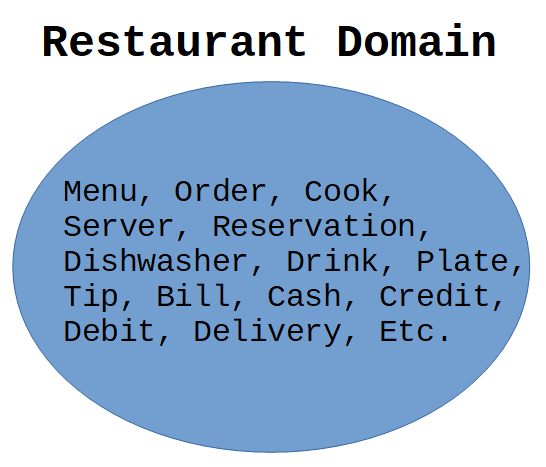
\includegraphics[width=.5\textwidth]{domain}
 \label{fig:domain}
\end{figure}

DDD requires the decomposition of the Domain into Subdomains, which facilitates our understanding. Subdomains are created by grouping related ideas, actions and rules. Some concepts may exist in multiple subdomains but they \emph{may not be the same}. In the Restaurant's Domain lets look at the \emph{Customer} concept:
\begin{itemize}
    \item Shared concepts (Customer) may not be identical initially;
    \item They may also look identical initially but them evolve differently over time. So we should avoid abstraction of the concept;
    \item Customer in the Reservation Subdomain (Figure~\ref{fig:subdomain}) may have details that are important in other part of the business.
\end{itemize}

Each Subdomain ends up having its own Ubiquitous Language and Model. The language and model for a subdomain is called a \emph{Bounded Context}.

\begin{figure}[ht]
\caption{Example of a Restaurant Reservation Subdomain}
\centering
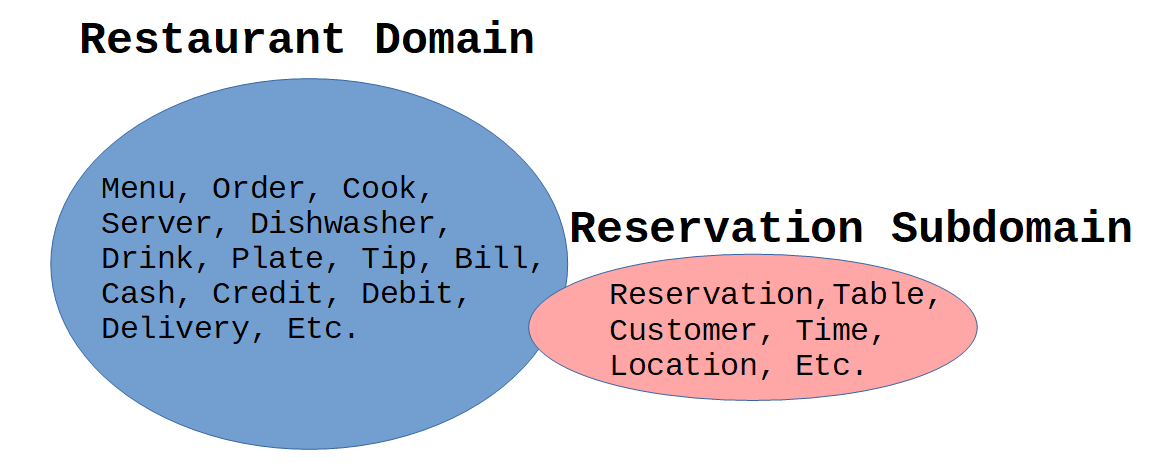
\includegraphics[width=1\textwidth]{subdomain}
 \label{fig:subdomain}
\end{figure}

\section{Bounded Contexts}

A Bounded Context is a logical boundary of a domain where particular terms and rules apply consistently. Inside this boundary, all terms, definitions, and concepts form the Ubiquitous Language. Taking the Restaurant Example we can define the following bounded context:
\begin{itemize}
    \item A customer in the Reservations Context will probably need to include certain details, eg phone number;
    \item Might not need to know the address, but in the Deliveries Context the address must be required;
    \item The model for a Customer in Reservations would likely not be the same as a model of a customer in other parts of the business;
    \item \emph{Bounded Context} is the combination of the \emph{Model} and the \emph{Ubiquitous Language};
    \item Subdomains and Bounded Contexts usually map in a kind of 1 to 1 relationship;
    \item Subdomains or Bounded Context are good starting points for building Reactive Microservices;
    \item Generally don't want all our bounded contexts built into a single service\footnote{With this approach you are building a monolith.}. 
\end{itemize}

\paragraph{Understanding Bounded Contexts}

From one Bounded Context to the meaning of a concept may change dramatically.
\begin{itemize}
    \item In a restaurant when talking to a server, an \emph{Order} has a very specific meaning. The client is the Customer;
    \item When speaking to the person who manages inventory for the restaurant \emph{Order} means something completely different. Restaurant is the Customer.
\end{itemize}

We also need to observe how the details of the model change.
\begin{itemize}
    \item In a restaurant, when the kithen is preparing an Order they don't care about prices;
    \item When a customer pays for the Order, price is critical;
    \item It is the same Order but the relevant details of that Order change;
    \item Depending in what part of the business, we are working in, the details of an Order will change.
\end{itemize}

\paragraph{Guidelines to determine Bounded Contexts}

\begin{itemize}
    \item Consider human interaction. Different areas of the domain that are handled by different groups of people, suggests a natural division. Might imply separate Bounded Context;
    \item Look for change in the Ubiquitous Language. If the use of language or the meaning of that language changes, that may suggest a new context (The Order that the server takes versus the Order for inventory.);
    \item Look for varying or unnecessary information (EmployeeId is very important in an Employee but meaningless in a Customer.);
    \item Strongly separated Bounded Contexts will result in smooth workflows. An awkward workflow may signal a misunderstanding of the domain, or that you've broken up your Domain / Bounded Context incorrectly;
    \item If a Bounded Context has too many dependencies it may be overcomplicated, you may have drawn the separation lines (subdomains) incorrectly.
\end{itemize}

You can find a real example of a Bounded Context in the Figure~\ref{fig:bounded}

\begin{figure}[ht]
\caption{Real division of a Domain}
\centering
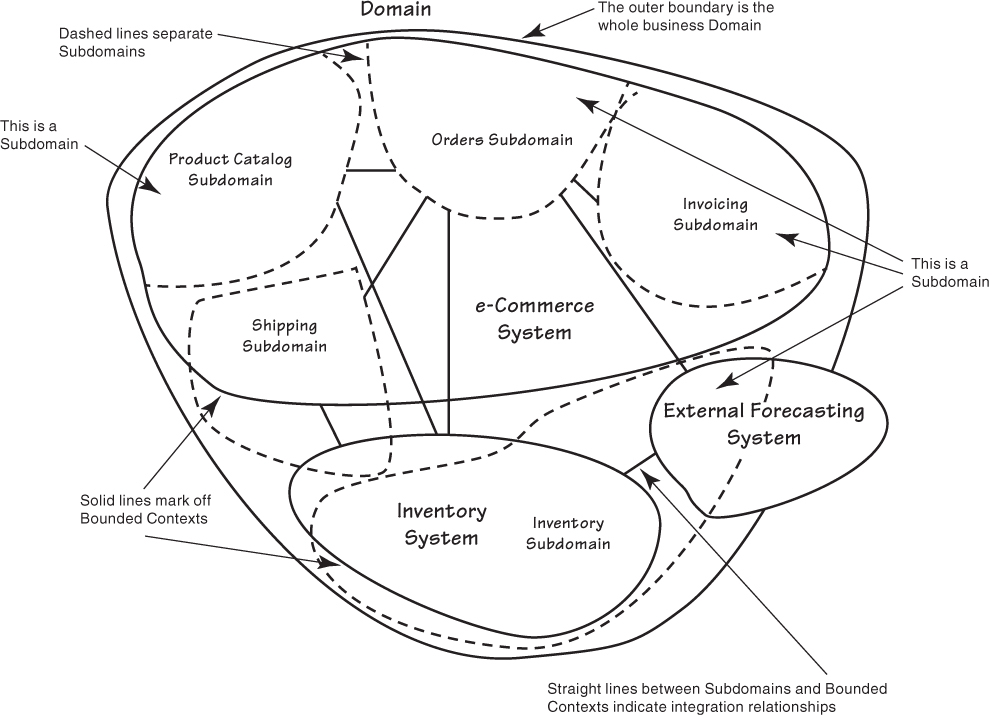
\includegraphics[width=1\textwidth]{bounded}
 \label{fig:bounded}
\end{figure}

\section{Strategies to Define the DDD Model}

\subsection{Event First Domain Driven Design}

Traditionally, DDD focused on the objects within the Domain. In more recent times, the techniques have evolved a bit and now we have \emph{Event First DDD} or \emph{Event Storming}. Event First DDD places the focus on the activities or events that occur in the domain. Eg.
\begin{itemize}
    \item Customer makes a reservation;
    \item Server places an order;
    \item Food is served to the customer.
\end{itemize}

Using Event First DDD, we start by defining the activities, then group those activities to find logical system boundaries.

\paragraph{Subject--Verb--Object Notation}
Subject--Verb--Object Notation provide us a consistent way to phrase our activities or events in the domain.
The sentences are composed by the subject first, the object as last and the verb in the middle. Example:

\begin{quote}
    Host checks current reservation.
\end{quote}
\begin{description}
    \item[Subject] Host;
    \item[Object] Reservation;
    \item[Verb] Check.
\end{description}

Note that \emph{current} is just a simple modifier on the object.

\paragraph{Direct versus Indirect Objects}

Lets look at the following sentence:
\begin{quote}
    Bartender collects Payment for a Drink Order.
\end{quote}

So, is \emph{Payment} or \emph{Order} the Object? 
In this context:
\begin{itemize}
    \item Payment is the Direct Object;
    \item Drink Order is the Indirect Object.
\end{itemize}

So they are \emph{both} Objects. We're less concerned with direct and indirect but we need to be aware that there will be often be more than one object. 

\subsection{Event Storming}

Event Storming is a workshop format for quickly exploring complex business domains. It is:
\begin{description}
    \item[Powerful] Allow many practitioners to come up with a comprehensive model of a complete business flow in hours instead weeks;
    \item[Engaging] The whole idea is to bring people with the questions and people who know the answer in the same room and to build a model together;
    \item[Efficient] The resulting model is perfectly align with the DDD model (particularly Event Sourcing) and allows for a quick determination of Context and Aggregate boundaries;
    \item[Easy] The notation is ultra-simple. No complex UML that cut off participants from the heart of the discussion.
    \item[Fun] People are energized and deliver more than they expected.
\end{description}

You can find more about event storm information in the Section \ref{chp2references} in the \cite{wiksto20} and \cite{albbra13} items.

\begin{figure}[ht]
\caption{Event Storming Layout}
\centering
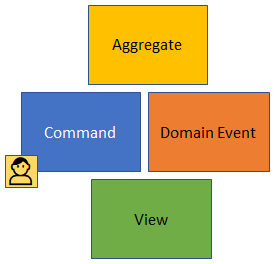
\includegraphics[width=.5\textwidth]{storming.png}
 \label{fig:storming}
\end{figure}

\section{Anti-Corruption Layers}
Anti-Corruption Layers (ACL) is a pattern that implements a fa\c cade or adapter layer between different subsystems that don't share the same semantics. 
This pattern is exemplified on the Figure~\ref{fig:aclfull}. So the goal of using ACLs is keep the clarity and purity between our Bounded Contexts. It's important to recognize that:
\begin{itemize}
    \item Each Bounded Contexts may have domain concepts that are unique. In the Figure~\ref{fig:acl}, we have the reservations context and our customer context. There are certain aspects of a Customer that are unique to the Customer Context. There are certain aspects of a customer that are unique to the customer, they don't matter to the reservation (eg. Address);
    \item Concepts are not always compatible from one context to the next. Sometimes, what happens is that you end up with a concept that is called one thing in the reservations context and called another thing in the customer context, or may end up with a situation where something is not compatible in such a way that it requires a translation of some kind (different units for example);
    \item Anti-Corruption Layers introduced to translate these concepts;
    \item ACL will prevent Bounded Contexts from leaking into each other: 
    \begin{itemize}
        \item Don't want to just come up with an abstraction or some way to make it the same across all Bounded Contexts;
        \item This would create coupling, that we need to avoid. Would need to make updates everywhere across all contexts, for minor changes in one.
    \end{itemize}
    \item ACLs help the Bounded Context to stand alone. It looks at whatever that Customer Context representation is and it translates it into a representation that is unique to the reservation service. Strips out unnecessary info like address in this case. This therefore maintains purity in the Reservation Context. This prevents leakage between Bounded Contexts;
    \item Standing alone. If we have a caching layer inside of the ACL, in case of failure, the service can be able to operate.
\end{itemize}

To implement the Anti-Corruption Layer we commonly use an Abstract Interface.
\begin{itemize}
    \item Interface represents the pure domain representation of the data;
    \item Implementation of the interface does the necessary translation.
\end{itemize}

\begin{figure}[ht]
\caption{Anti-Corruption Layer}
\centering
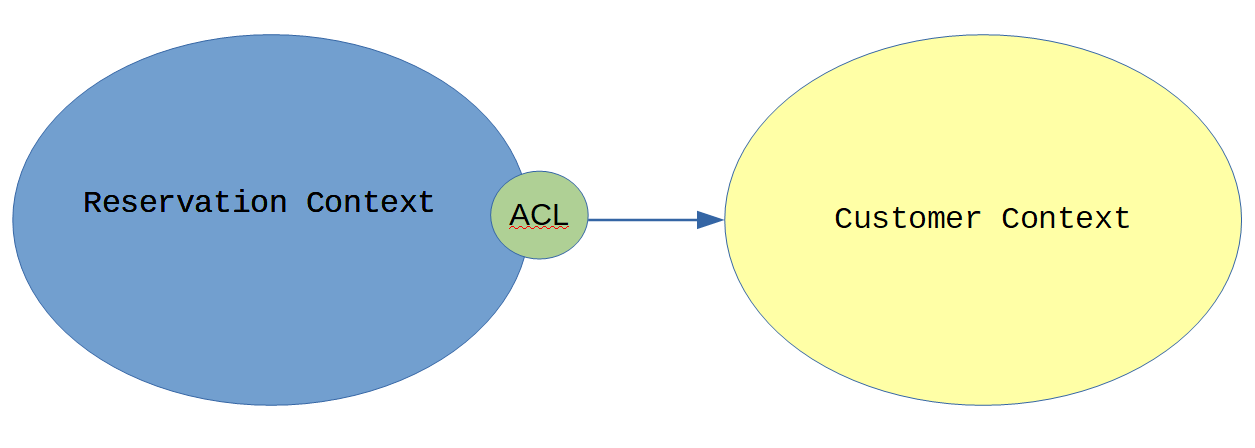
\includegraphics[width=1\textwidth]{acl}
 \label{fig:acl}
\end{figure}


\begin{figure}[ht]
\caption{Anti-Corruption Layer Example}
\centering
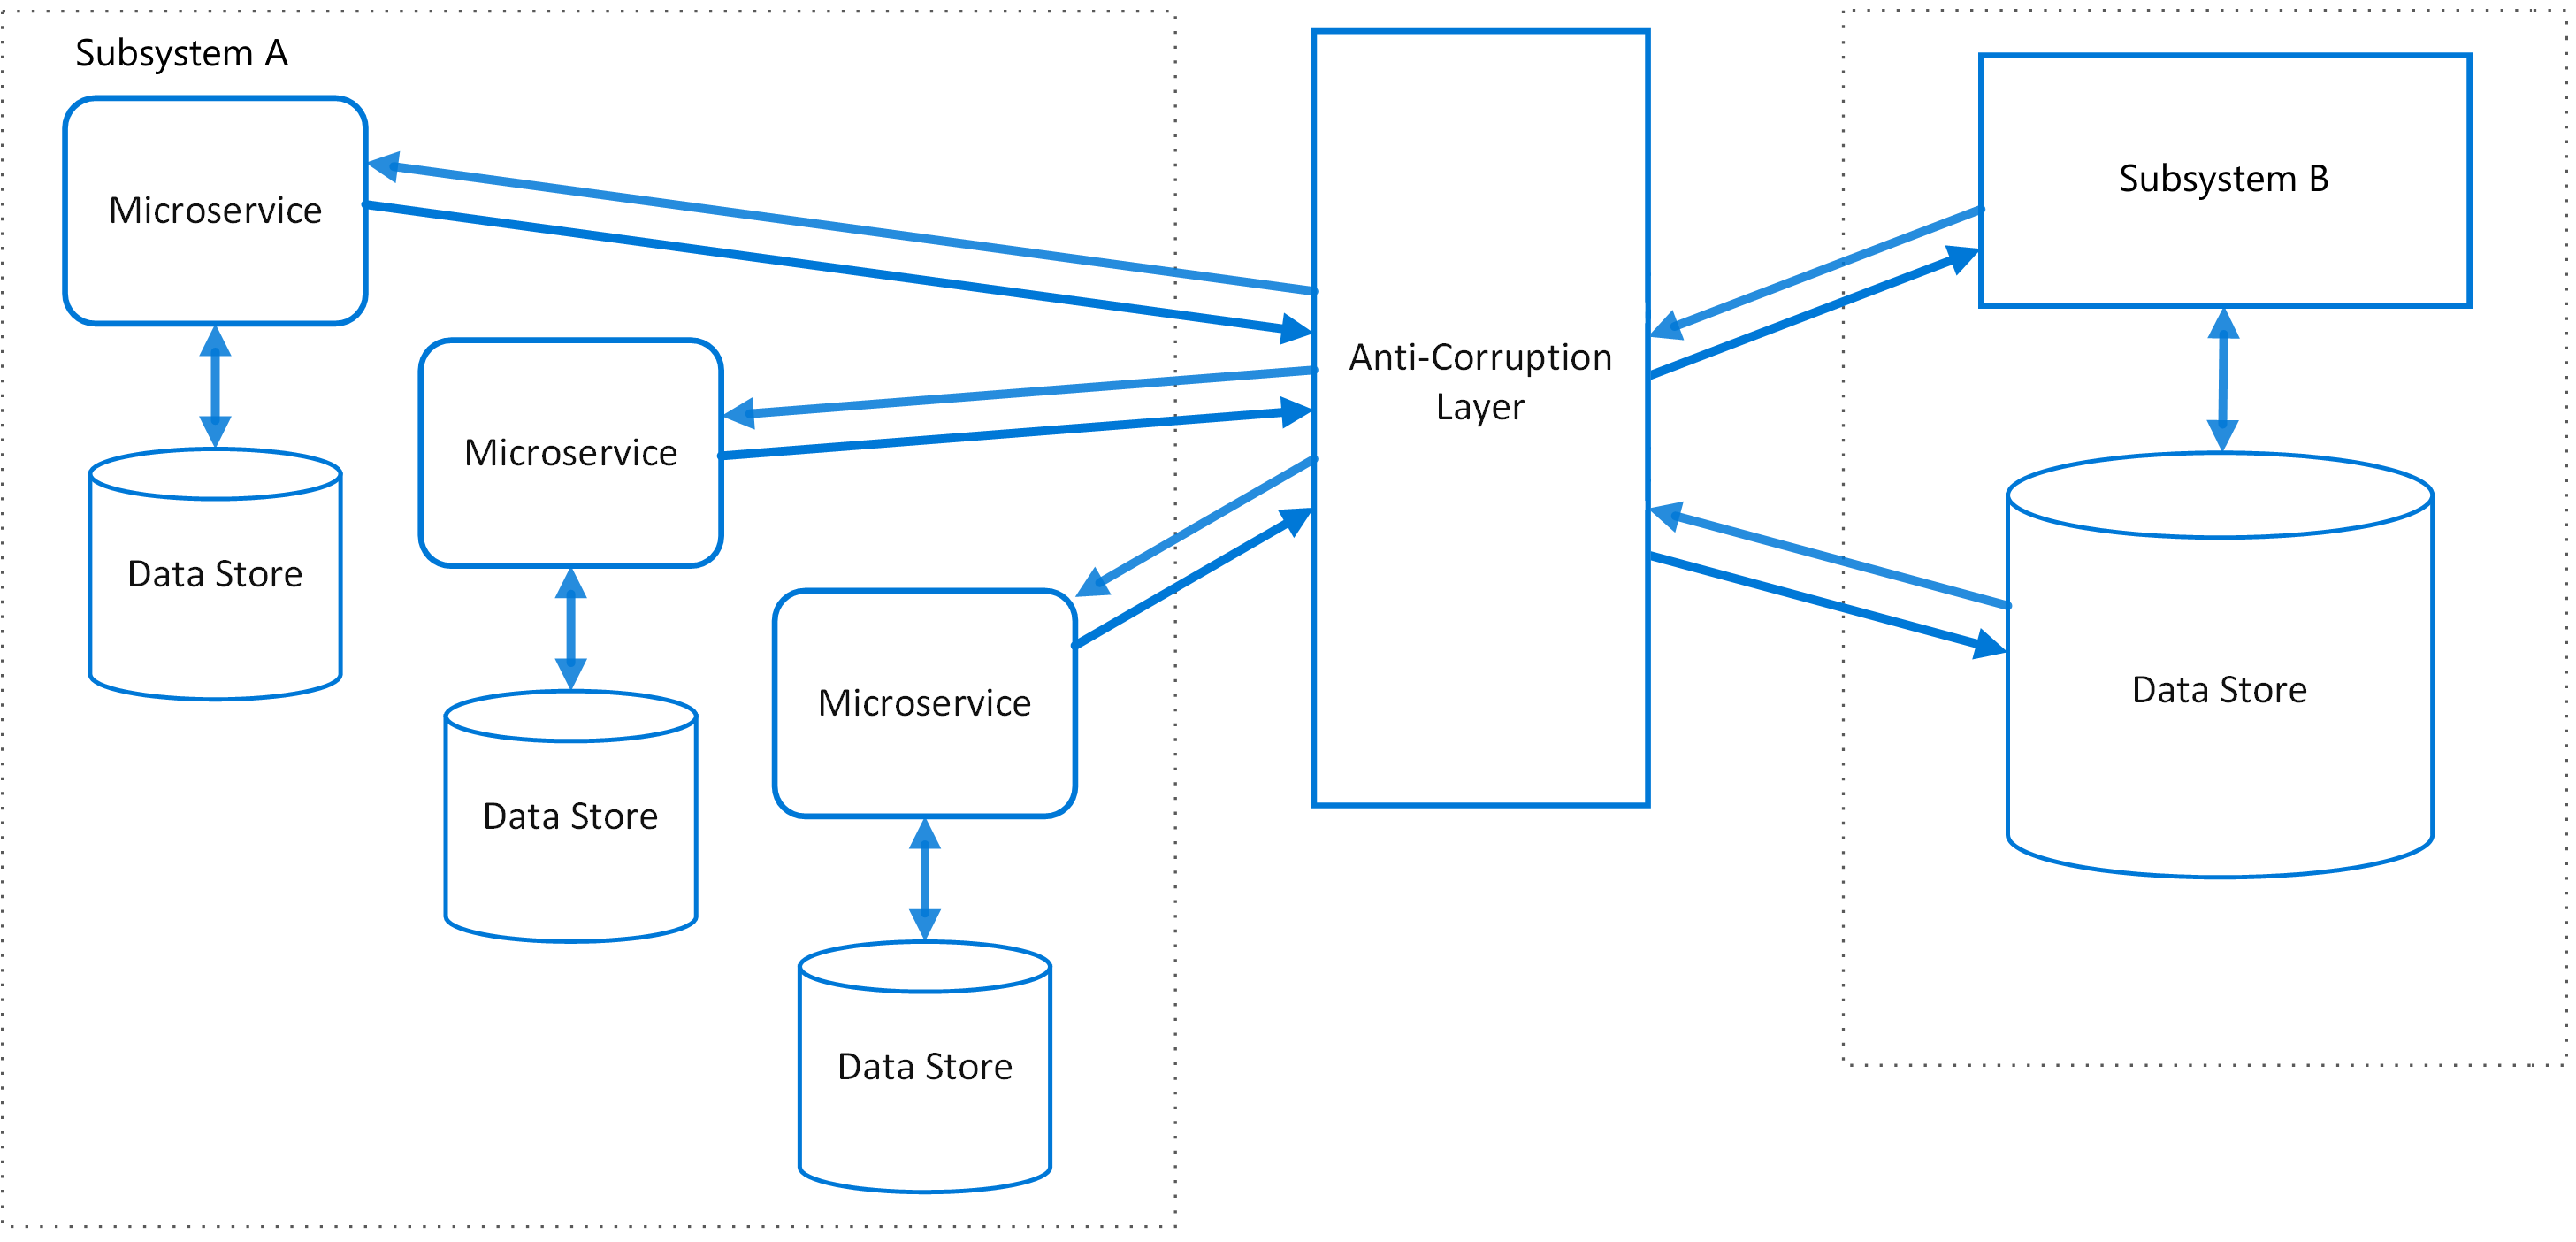
\includegraphics[width=1\textwidth]{anti-corruption-layer}
 \label{fig:aclfull}
\end{figure}

\subsection{Anti-Corruption Layer for Legacy Systems}

Organizations often choose to integrate legacy systems with their replacements, either for the short term or indefinitely. But there's a risk: connecting the old to the new can drag unwanted problems into what is a clean design. Legacy systems suffer from outdated protocols, data models, schemas and/or obsolete APIs. To interface legacy systems, new(er) pipeline applications may need to support legacy features that don't align with modern architectural techniques. Based in the example in the Figure~\ref{fig:acllegacy}, ACLs can help with:
\begin{itemize}
    \item In this case, the domain may be messy or unclear, ACL has the job of keeping the mess of that legacy system out of our pure Bounded Context;
    \item Keeps our Bounded Context pure;
    \item Prevents our domain from having to deal with the mess;
    \item ACL may be implemented in the Legacy System, or in the Bounded Context, or Both as the example provided;
    \item It's recommended that every time a pure microservice or a Pure Bounded Context has to communicate with another external service of some kind, it should do throught an ACL;
    \item With the legacy service, because of the complexity of it, may want to expose an API that's just for the Reservations Context which then has a bit cleaner that what the messy legacy system would typically be exposing.
\end{itemize}

\begin{figure}[ht]
\caption{Anti-Corruption Layer for Legacy Systems}
\centering
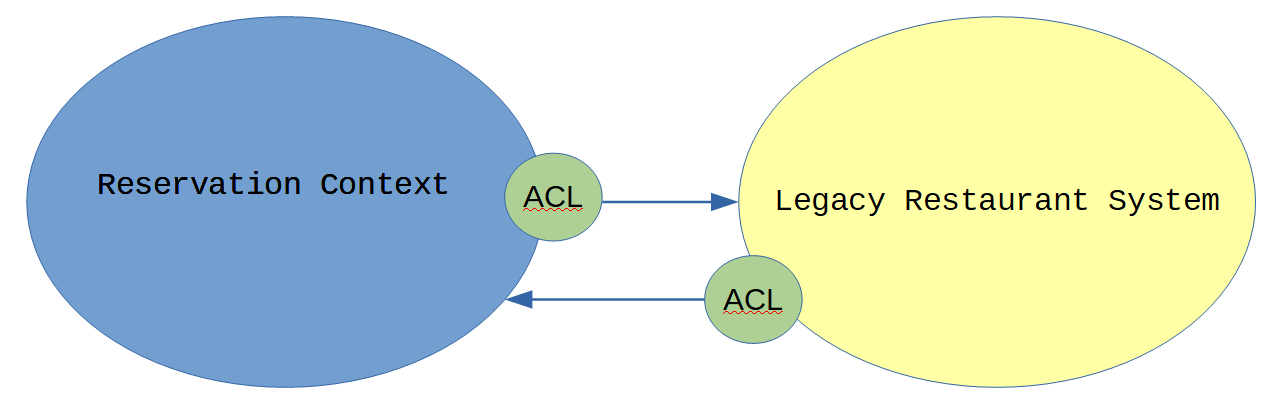
\includegraphics[width=1\textwidth]{acl_legacy}
 \label{fig:acllegacy}
\end{figure}

\section{Context Maps}

\section{Domain Activities}

\subsection{Commands}

\subsection{Events}

\subsection{Queries}

\section{Domain Objects}

\subsection{Values}

\subsection{Entities}

\subsection{Aggregates}

\section{Domain Abstractions}

\subsection{Services}

\subsection{Factories}

\subsection{Repositories}

\section{Hexagonal Architecture}

\section{References} \label{chp2references}

\begin{thebibliography}{9}

\bibitem{wiksto20}
Wikipedia,
\href{https://en.wikipedia.org/wiki/Event_storming}{\textit{Event Storming}}, 
2020

\bibitem{albbra13}
Alberto Brandolini,
\href{http://ziobrando.blogspot.com/2013/11/introducing-event-storming.html}{\textit{Introducing Event Storming}}, 
2013

\end{thebibliography}
